\chapter{Control \& Status Registers}\label{control-status-registers}

\section{Introduction}\label{introduction-3}

The state of the CPU is maintained by the Control \& Status Registers
(CSRs). They determine the feature set, set interrupts and interrupt
masks, and determine the privilege level. The CSRs are mapped into an
internal 12bit address space and are accessible using special commands.

\section{Accessing the CSRs}\label{accessing-the-csrs}

\missingfigure{}

Figure ‑: CSR Instructions

The CSRRW (Atomic Read/Write CSR) instruction atomically swaps values in
the CSRs and integer registers. CSRRW reads the old value of the CSR,
zero-extends the value to XLEN bits, and writes it to register
\emph{rd}. The initial value in register \emph{rs1} is written to the
CSR.

The CSRRS (Atomic Read and Set CSR) instruction reads the old value of
the CSR, zero-extends the value to XLEN bits, and writes it to register
\emph{rd}. The initial value in register \emph{rs1} specifies the bit
positions to be set in the CSR. Any bit that is high in \emph{rs1} will
be set in the CSR, assuming that bit can be set. The effect is a logic
OR between the old value in the CSR and the new value in \emph{rs1}.

If \emph{rs1}=X0, then the CSR is not written to.

The CSRRC (Atomic Read and Clear CSR) instruction reads the old value of
the CSR, zero-extends the value to XLEN bits, and writes it to register
\emph{rd}. The initial value in register \emph{rs1} specifies the bit
positions to be cleared in the CSR. Any bit that is high in \emph{rs1}
will be cleared in the CSR, assuming that bit can be cleared. If
\emph{rs1}=X0, then the CSR is not written to.

The CSRRWI, CSRRSI, and CSRRCI commands are similar in behavior. Except
that they update the CSR using an immediate value, instead of
referencing a source register. The immediate value is obtained by
zero-extending the 5bit \emph{zimm} field. If \emph{zimm{[}4:0{]}} is
zero, then the CSR is not written to.

\section{Illegal CSR accesses}\label{illegal-csr-accesses}

Depending on the privilege level some CSRs may not be accessible.
Attempts to access a non-existing CSR raise an illegal-instruction
exception. Attempts to access a privileged CSR or write a read-only CSR
raise an illegal-instruction exception. Machine Mode can access all
CSRs, whereas User Mode can only access a
few.

\section{Timers and Counters}\label{timers-and-counters}

\missingfigure{}

Table ‑: Time \& Counter Instructions

The RV12 provides a number of 64-bit read-only user-level counters,
which are mapped into the 12-bit CSR address space and accessed in
32-bit pieces using CSRRS instructions.

The RDCYCLE pseudo-instruction reads the low XLEN bits of the cycle CSR
that holds a count of the number of clock cycles executed by the
processor on which the hardware thread is running from an arbitrary
start time in the past. RDCYCLEH is an RV32I-only instruction that reads
bits 63--32 of the same cycle counter. The rate at which the cycle
counter advances will depend on the implementation and operating
environment.

The RDTIME pseudo-instruction reads the low XLEN bits of the time CSR,
which counts wall-clock real time that has passed from an arbitrary
start time in the past. RDTIMEH is an RV32I-only instruction that reads
bits 63--32 of the same real-time counter. The underlying 64-bit counter
should never overflow in practice. The execution environment should
provide a means of determining the period of the real-time counter
(seconds/tick). The period must be constant. The real-time clocks of all
hardware threads in a single user application should be synchronized to
within one tick of the real-time clock. The environment should provide a
means to determine the accuracy of the clock.

The RDINSTRET pseudo-instruction reads the low XLEN bits of the instret
CSR, which counts the number of instructions retired by this hardware
thread from some arbitrary start point in the past. RDINSTRETH is an
RV32I-only instruction that reads bits 63--32 of the same instruction
counter.

In RV64I, the CSR instructions can manipulate 64-bit CSRs. In
particular, the RDCYCLE, RDTIME, and RDINSTRET pseudo-instructions read
the full 64 bits of the cycle, time, and instret counters. Hence, the
RDCYCLEH, RDTIMEH, and RDINSTRETH instructions are not necessary and are
illegal in RV64I.

\section{CSR Listing}\label{csr-listing}

The following sections describe each of the register functions as
specifically implemented in RV12.

Note: These descriptions are derived from ``The RISC-V Instruction Set
Manual, Volume II: Privileged Architecture, Version 1.9.1", Editors
Andrew Waterman and Krste Asanović, RISC-V Foundation, November 4, 2016,
and released under the Creative Commons Attribution 4.0 International
License

\begin{longtable}[]{@{}cccl@{}}
\toprule
\textbf{Address} & \textbf{Privilege} & \textbf{Name} & \textbf{Description}\tabularnewline
\midrule
\endfirsthead
\multicolumn{4}{c}{{(Continued from previous page)}} \\
\toprule
\textbf{Address} & \textbf{Privilege} & \textbf{Name} & \textbf{Description}\tabularnewline
\midrule
\endhead
\midrule \multicolumn{4}{c}{{\tablename\ \thetable{} continued on next page\ldots}} \\
\endfoot
\endlastfoot

\rowcolor{rltable}\multicolumn{4}{c}{\emph{\textbf{Machine Information Registers}}}\tabularnewline
0xF11 & MRO & \texttt{mvendorid} & Vendor ID\tabularnewline
0xF12 & MRO & \texttt{marchid}   & Architecture ID\tabularnewline
0xF13 & MRO & \texttt{mimpid}    & Implementation ID\tabularnewline
0xF14 & MRO & \texttt{mhartid}   & Hardware thread ID\tabularnewline

\rowcolor{rltable}\multicolumn{4}{c}{\emph{\textbf{Machine Trap Setup}}}\tabularnewline
0x300 & MRW & \texttt{mstatus} & Machine status register\tabularnewline
0x301 & MRW & \texttt{misa}    & ISA and extensions\tabularnewline
0x302 & MRW & \texttt{medeleg} & Machine exception delegation register\tabularnewline
0x303 & MRW & \texttt{mideleg} & Machine interrupt delegation register\tabularnewline
0x304 & MRW & \texttt{mie}     & Machine interrupt-enable register\tabularnewline
0x305 & MRW & \texttt{mtvec}   & Machine trap-handler base address\tabularnewline
0x7c0 & MRW & \texttt{mnmivec} & Machine non-maskable interrupt vector\tabularnewline

\rowcolor{rltable}\multicolumn{4}{c}{\emph{\textbf{Machine Trap Handling}}}\tabularnewline
0x340 & MRW & \texttt{mscratch} & Scratch register for machine trap handler\tabularnewline
0x341 & MRW & \texttt{mepc}     & Machine exception program counter\tabularnewline
0x342 & MRW & \texttt{mcause}   & Machine trap cause\tabularnewline
0x343 & MRW & \texttt{mbadaddr} & Machine bad address\tabularnewline
0x344 & MRW & \texttt{mip}      & Machine interrupt pending\tabularnewline

\rowcolor{rltable}\multicolumn{4}{c}{\emph{\textbf{Machine Counter/Timers}}}\tabularnewline
0xB00 & MRW & \texttt{mcycle}    & Machine cycle counter\tabularnewline
0xB02 & MRW & \texttt{minstret}  & Machine instructions-retired counter\tabularnewline
0xB80 & MRW & \texttt{mcycleh}   & Upper 32 bits of \texttt{mcycle}, RV32I only\tabularnewline
0xB82 & MRW & \texttt{minstreth} & Upper 32 bits of \texttt{minstret}, RV32I only\tabularnewline
\bottomrule
\caption{Machine Mode CSRs}
\label{tab:machine-csrs}
\end{longtable}


\begin{longtable}[]{@{}cccl@{}}
\toprule
\textbf{Address} & \textbf{Privilege} & \textbf{Name} & \textbf{Description}\tabularnewline
\midrule
\endfirsthead
\multicolumn{4}{c}{{(Continued from previous page)}} \\
\toprule
\textbf{Address} & \textbf{Privilege} & \textbf{Name} & \textbf{Description}\tabularnewline
\midrule
\endhead
\midrule \multicolumn{4}{c}{{\tablename\ \thetable{} continued on next page\ldots}} \\
\endfoot
\endlastfoot

\multicolumn{4}{c}{\emph{\textbf{Supervisor Trap Handling}}}\tabularnewline
0x100 & SRW & \texttt{sstatus} & Supervisor status register\tabularnewline
0x102 & SRW & \texttt{sedeleg} & Supervisor exception delegation register\tabularnewline
0x103 & SRW & \texttt{sideleg} & Supervisor interrupt delegation register\tabularnewline
0x104 & SRW & \texttt{sie}     & Supervisor interrupt-enable register\tabularnewline
0x105 & SRW & \texttt{stvec}   & Supervisor trap handler base address\tabularnewline

\multicolumn{4}{c}{\emph{\textbf{Supervisor Trap Handling}}}\tabularnewline
0x140 & SRW & \texttt{sscratch} & Scratch register for trap handler\tabularnewline
0x141 & SRW & \texttt{sepc}     & Supervisor exception program counter\tabularnewline
0x142 & SRO & \texttt{scause}   & Supervisor trap cause\tabularnewline
0x143 & SRO & \texttt{sbadaddr} & Supervisor bad address\tabularnewline
0x144 & SRW & \texttt{sip}      & Supervisor interrupt pending register\tabularnewline
\bottomrule
\caption{Supervisor Mode CSRs}
\label{tab:supervisor-csrs}
\end{longtable}


\begin{longtable}[]{@{}cccl@{}}
\toprule
\textbf{Address} & \textbf{Privilege} & \textbf{Name} & \textbf{Description}\tabularnewline
\midrule
\endfirsthead
\multicolumn{4}{c}{{(Continued from previous page)}} \\
\toprule
\textbf{Address} & \textbf{Privilege} & \textbf{Name} & \textbf{Description}\tabularnewline
\midrule
\endhead
\midrule \multicolumn{4}{c}{{\tablename\ \thetable{} continued on next page\ldots}} \\
\endfoot
\endlastfoot

\multicolumn{4}{c}{\emph{\textbf{User Counter / Timers}}}\tabularnewline
0xC00 & URO & \texttt{cycle} & Cycle counter for \texttt{RDCYCLE} instruction\tabularnewline
0xC02 & URO & \texttt{instret} & Instruction-retire counter for \texttt{RDINSTRET}\tabularnewline
0xC80 & URO & \texttt{cycleh} & Upper 32bits of \texttt{cycle}, RV32I only\tabularnewline
0xC82 & URO & \texttt{instret} h& Upper 32bit of \texttt{instret}, RV32I only\tabularnewline
\bottomrule
\caption{User Mode CSRs}
\label{tab:user-csrs}
\end{longtable}

\section{Machine Level CSRs}\label{machine-level-csrs}

In addition to the machine-level CSRs described in this section, M-mode
can access all CSRs at lower privilege levels.

\subsection{Machine ISA Register
(misa)}\label{machine-isa-register-misa}

The misa register is an XLEN-bit WARL read-write register reporting the
ISA supported by the hart.

\missingfigure{}


Figure ‑: Machine ISA Register Format

The extensions field encodes the presence of the standard extensions,
with a single bit per letter of the alphabet (bit 0 encodes the presence
of extension ``A'', bit 1 encodes the presence of extension ``B'',
through to bit 25 that encodes the presence of extension ``Z'').

The ``I'' bit will be set for RV32I and RV64I base ISAs, and the ``E''
bit will be set for RV32E.

The Base field encodes the native base integer ISA width as shown in
Table 7‑5.

\begin{longtable}[]{@{}cc@{}}
\toprule
Value & Description\tabularnewline
\midrule
\endhead
1 & 32\tabularnewline
2 & 64\tabularnewline
\bottomrule
\caption{Supported misa values}
\label{tab:misa-values}
\end{longtable}

\subsection{Vendor ID Register
(mvendorid)}\label{vendor-id-register-mvendorid}

The mvendorid read-only register is an XLEN-bit register encoding the
manufacturer of the device.

\begin{figure}[hbt]
  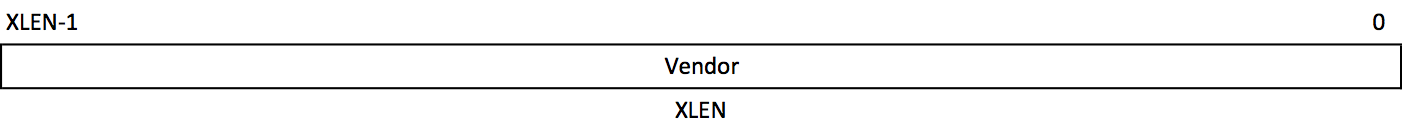
\includegraphics[width=\textwidth]{mvendorid}
  \caption{Vendor ID Register}
\end{figure}


Figure ‑: Vendor ID Register

Non-Zero vendor IDs will be allocated by the RISC-V Foundation.

\subsection{Architecture ID Register
(marchid)}\label{architecture-id-register-marchid}

The marched CSR is an XLEN-bit read-only register encoding the base
microarchitecture of the hart. For the RV12 CPU this is defined as shown
in Figure 7‑5.

\begin{figure}[hbt]
  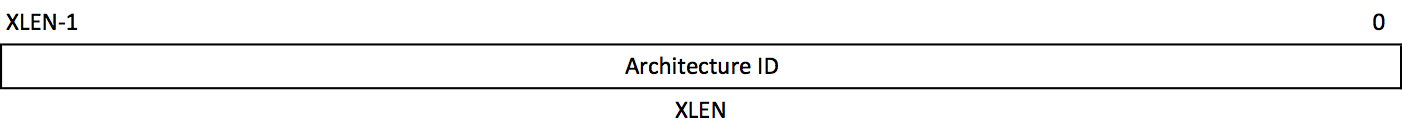
\includegraphics[width=\textwidth]{marchid}
  \caption{Architecture ID Register}
\end{figure}

Note: Open-source project architecture IDs are allocated globally by the
RISC-V Foundation, and have non-zero architecture IDs with a zero
most-significant-bit (MSB). Commercial architecture IDs are allocated by
each commercial vendor independently and have the MSB set.

\subsection{Implementation ID Register
(mimpid)}\label{implementation-id-register-mimpid}

The mimpid read-only register provides hardware version information for
the CPU. In the Roa Logic implementation, the 2 least significant bytes
encode the major and minor code revisions.

\begin{figure}[hbt]
  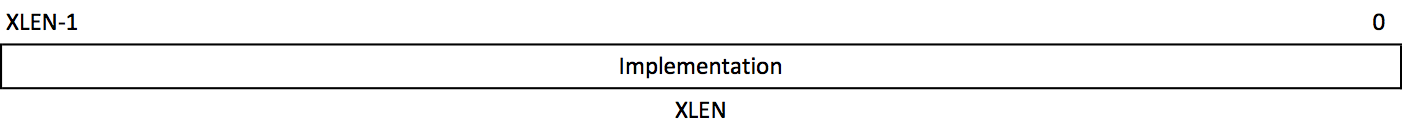
\includegraphics[width=\textwidth]{mimpid}
  \caption{Roa Logic mimpid}
\end{figure}

The mimpid register is an XLEN size register, but the RV12 only
implements the lower 32 bits. For an RV64 implementation the MSBs are
zero extended.

\subsection{Hardware Thread ID Register
(mhartid)}\label{hardware-thread-id-register-mhartid}

\missingfigure{}

Figure ‑: Hardware Thread ID Register

The mhartid read-only register indicates the hardware thread that is
running the code. The RV12 implements a single thread, therefore this
register always reads zero.

\subsection{Machine Status Register
(mstatus)}\label{machine-status-register-mstatus}

The mstatus register is an XLEN-bit read/write register that keeps track
of and controls the \emph{hart's} current operating state.

\subsubsection{Privilege and Global Interrupt-Enable Stack in mstatus register}

Interrupt-enable bits, MIE, SIE, and UIE, are provided for each
privilege mode. These bits are primarily used to guarantee atomicity
with respect to interrupt handlers at the current privilege level. When
a hart is executing in privilege mode \emph{x}, interrupts are enabled
when \emph{x}IE=1. Interrupts for lower privilege modes are always
disabled, whereas interrupts for higher privilege modes are always
enabled. Higher-privilege-level code can use separate per-interrupt
enable bits to disable selected interrupts before ceding control to a
lower privilege level.

\missingfigure{}

Figure ‑: Machine Mode Status Register

The MRET, SRET, or URET instructions are used to return from traps in
M-mode, S-mode, or U-mode respectively. When executing an \emph{x}RET
instruction, supposing \emph{x}PP holds the value \emph{y}, \emph{y}IE
is set to \emph{x}PIE; the privilege mode is changed to \emph{y};
\emph{x}PIE is set to 1; and \emph{x}PP is set to U.

\subsubsection{Memory Privilege in mstatus Register
}\label{memory-privilege-in-mstatus-register}

The MPRV bit modifies the privilege level at which loads and stores
execute. When MPRV='0', translation and protection behave as normal.
When MPRV='1', data memory addresses are translated and protected as
though PRV were set to the current value of the PRV1 field. Instruction
address-translation and protection are unaffected. When an exception
occurs, MPRV is reset to 0.

\subsubsection{Virtualization Management \& Context Extension Fields in
mstatus Register
}\label{virtualization-management-context-extension-fields-in-mstatus-register}

Virtualization and Context Extensions are not supported by the RV12 v1.0
implementation. The value of these fields will therefore be permanently
set to 0.

\subsection{Machine Delegation Registers
(medeleg \& mideleg)} \label{machine-exception-interrupt-delegation-registers-medeleg-mideleg}

Individual read/write bits within medeleg and mideleg registers indicate
that lower privilege levels should directly process certain exceptions
and interrupts.

When a trap is delegated to a less-privileged mode \emph{x}, the
\emph{x}cause register is written with the trap cause; the \emph{x}epc
register is written with the virtual address of the instruction that
took the trap; the \emph{x}PP field of mstatus is written with the
active privilege mode at the time of the trap; the \emph{x}PIE field of
mstatus is written with the value of the active interrupt-enable bit at
the time of the trap; and the \emph{x}IE field of mstatus is cleared.
The mcause and mepc registers and the MPP and MPIE fields of mstatus are
not written.

\missingfigure{}

Figure ‑: Machine Exception
Delegation Register

medeleg has a bit position allocated for every synchronous exception
shown in Table 7‑8, with the index of the bit position equal to the
value returned in the mcause register (I.e. setting bit 8 allows
user-mode environment calls to be delegated to a lower-privilege trap
handler). See section 7.6.13 for additional details.

\missingfigure{}

\protect\hypertarget{_Ref367088721}{}{}Figure ‑: Machine Interrupt
Delegation Register

mideleg holds trap delegation bits for individual interrupts, with the
layout of bits matching those in the mip register (I.e. STIP interrupt
delegation control is located in bit 5).

\subsection{Machine Interrupt Registers (mie \&
mip)}\label{machine-interrupt-registers-mie-mip}

The mip register is an XLEN-bit read/write register containing
information on pending interrupts, while mie is the corresponding
XLEN-bit read/write register containing interrupt enable bits. Only the
bits corresponding to lower-privilege software interrupts (USIP, SSIP)
and timer interrupts (UTIP, STIP) in mip are writable through this CSR
address; the remaining bits are read-only.

Restricted views of the mip and mie registers appear as the sip/sie, and
uip/uie registers in S-mode, and U-mode respectively. If an interrupt is
delegated to privilege mode \emph{x} by setting a bit in the mideleg
register, it becomes visible in the \emph{x}ip register and is maskable
using the \emph{x}ie register. Otherwise, the corresponding bits in
\emph{x}ip and \emph{x}ie appear to be hardwired to zero.

\missingfigure{}

Figure ‑: Machine Interrupt Pending Register

\missingfigure{}
Figure ‑: Machine Interrupt Enable Register

The MTIP, STIP, UTIP bits correspond to timer interrupt-pending bits for
machine, supervisor, and user timer interrupts, respectively. The MTIP
bit is read-only and is cleared by writing to the memory-mapped
machine-mode timer compare register. The UTIP and STIP bits may be
written by M-mode software to deliver timer interrupts to lower
privilege levels. User and supervisor software may clear the UTIP and
STIP bits with calls to the AEE or SEE respectively.

There is a separate timer interrupt-enable bit, named MTIE, STIE, and
UTIE for M-mode, S-mode, and U-mode timer interrupts respectively.

Each lower privilege level has a separate software interrupt-pending bit
(SSIP, USIP), which can be both read and written by CSR accesses from
code running on the local hart at the associated or any higher privilege
level. The machine-level MSIP bits are written by accesses to
memory-mapped control registers, which are used by remote harts to
provide machine-mode interprocessor interrupts. Interprocessor
interrupts for lower privilege levels are implemented through ABI or SBI
calls to the AEE or SEE respectively, which might ultimately result in a
machine- mode write to the receiving hart's MSIP bit. A hart can write
its own MSIP bit using the same memory-mapped control register.

The MEIP, SEIP, UEIP bits correspond to external interrupt-pending bits
for machine, supervisor, and user external interrupts, respectively.
These bits are read-only and are set and cleared by a platform-specific
interrupt controller. There is a separate external interrupt-enable bit,
named MEIE, SEIE, and UEIE for M-mode, S-mode, and U-mode external
interrupts respectively.

An interrupt \emph{i} will be taken if bit \emph{i} is set in both mip
and mie, and if interrupts are globally enabled. By default, M-mode
interrupts are globally enabled if the hart's current privilege mode is
less than M, or if the current privilege mode is M and the MIE bit in
the mstatus register is set. If bit \emph{i} in mideleg is set, however,
interrupts are considered to be globally enabled if the hart's current
privilege mode equals the delegated privilege mode (S, or U) and that
mode's interrupt enable bit (SIE or UIE in mstatus) is set, or if the
current privilege mode is less than the delegated privilege mode.

Multiple simultaneous interrupts and traps at the same privilege level
are handled in the following decreasing priority order: external
interrupts, software interrupts, timer interrupts, and then finally any
synchronous traps.

\subsection{Machine Trap-Handler Base Address Register
(mtvec)}\label{machine-trap-handler-base-address-register-mtvec}

The mtvec register is an XLEN-bit read/write register that holds the
base address of the M-mode trap vector.

\missingfigure{}

Figure ‑: Machine Trap-Handler Base Address Register

All traps into machine mode cause the pc to be set to the value in
mtvec. Additional trap vector entry points can be defined by
implementations to allow more rapid identification and service of
certain trap causes.

\subsection{Machine Non-Maskable Interrupt Vector
(mnmivec)}\label{machine-non-maskable-interrupt-vector-mnmivec}

The mnmivec register is an XLEN-bit read/write register that holds the
base address of the non-maskable interrupt trap vector. When an
exception occurs, the pc is set to mnmivec.

\missingfigure{}

Figure ‑: Machine Non-Maskable Interrupt Vector

\subsection{Machine Trap Handler Scratch Register
(mscratch)}\label{machine-trap-handler-scratch-register-mscratch}

The mscratch register is an XLEN-bit read/write register dedicated for
use by machine mode. It is used to hold a pointer to a machine-mode
hart-local context space and swapped with a user register upon entry to
an M-mode trap handler.

\missingfigure{}

Figure ‑: Machine-mode Scratch Register

\subsection{Machine Exception Program Counter Register
(mepc)}\label{machine-exception-program-counter-register-mepc}

mepc is an XLEN-bit read/write register. The two low bits
(mepc{[}1:0{]}) are always zero.

\missingfigure{}

Figure ‑: Machine Exception Program Counter Register

When a trap is taken, mepc is written with the virtual address of the
instruction that encountered the exception.

\subsection{Machine Trap Cause Register
(mcause)}\label{machine-trap-cause-register-mcause}

The mcause register is an XLEN-bit read-write register. The Interrupt
bit is set if the exception was caused by an interrupt. The Exception
Code field contains a code identifying the last exception. The remaining
center bits will read zero

\missingfigure{}

Figure ‑: Machine Cause Register

Table \ref{tab:mcause-reg-values} below lists the possible machine-level exception codes.

\begin{longtable}[]{@{}ccl@{}}
\toprule
Interrupt & Exception Code & Description\tabularnewline
\midrule
\endfirsthead
\multicolumn{3}{c}{{(Continued from previous page)}} \\

\toprule
Interrupt & Exception Code & Description\tabularnewline
\midrule
\endhead

\midrule \multicolumn{3}{c}{{\tablename\ \thetable{} continued on next page\ldots}} \\
\endfoot

\endlastfoot
1 & 0 & User software interrupt\tabularnewline
1 & 1 & Supervisor software interrupt\tabularnewline
1 & 2 & \emph{Reserved}\tabularnewline
1 & 3 & Machine software interrupt\tabularnewline
1 & 4 & User timer interrupt\tabularnewline
1 & 5 & Supervisor timer interrupt\tabularnewline
1 & 6 & \emph{Reserved}\tabularnewline
1 & 7 & Machine timer interrupt\tabularnewline
1 & 8 & User external interrupt\tabularnewline
1 & 9 & Supervisor external interrupt\tabularnewline
1 & 10 & \emph{Reserved}\tabularnewline
1 & 11 & Machine external interrupt\tabularnewline
1 & $\geqslant$12 & Reserved\tabularnewline
\midrule
0 & 0 & Instruction address misaligned\tabularnewline
0 & 1 & Instruction access fault\tabularnewline
0 & 2 & Illegal Instruction\tabularnewline
0 & 3 & Breakpoint\tabularnewline
0 & 4 & Load address misaligned\tabularnewline
0 & 5 & Load access fault\tabularnewline
0 & 6 & Store/AMO address misaligned\tabularnewline
0 & 7 & Store/AMO access fault\tabularnewline
0 & 8 & Environment call from U-mode\tabularnewline
0 & 9 & Environment call from S-mode\tabularnewline
0 & 10 & \emph{Reserved}\tabularnewline
0 & 11 & Environment call from M-mode\tabularnewline
0 & $\geqslant$12 & \emph{Reserved}\tabularnewline
\bottomrule
\caption{Machine Cause Register Values}
\label{tab:mcause-reg-values}
\end{longtable}


\subsection{Machine Bad Address Register
(mbadaddr)}\label{machine-bad-address-register-mbadaddr}

mbadaddr is an XLEN-bit read-write register. When a hardware breakpoint
is triggered, or an instruction-fetch, load, or store address-misaligned
or access exception occurs, mbadaddr is written with the faulting
address. mbadaddr is not modified for other exceptions.

\missingfigure{}

Figure ‑: Machine Bad Address Register

For instruction-fetch access faults with variable-length instructions,
mbadaddr will point to the portion of the instruction that caused the
fault while mepc will point to the beginning of the instruction.

\subsection{Machine Cycle Counter (mcycle,
mcycleh)}\label{machine-cycle-counter-mcycle-mcycleh}

The mcycle CSR holds a count of the number of cycles the hart has
executed since some arbitrary time in the past. The mcycle register has
64-bit precision on all RV32 and RV64 systems.

On RV32 only, reads of the mcycle CSR returns the low 32 bits, while
reads of the mcycleh CSR returns bits 63--32.

\subsection{Machine Instructions-Retired counter (minstret,
minstreth)}\label{machine-instructions-retired-counter-minstret-minstreth}

The minstret CSR holds a count of the number of instructions the hart
has retired since some arbitrary time in the past. The minstret register
has 64-bit precision on all RV32 and RV64 systems.

On RV32 only, reads of the minstret CSR returns the low 32 bits, while
reads of the minstreth CSR returns bits 63--32.

\section{Supervisor Mode CSRs}\label{supervisor-mode-csrs}

\subsection{Supervisor Status Register (sstatus)
}\label{supervisor-status-register-sstatus}

The sstatus register is an XLEN-bit read/write register formatted as
shown in Figure 7‑19. The sstatus register keeps track of the
processor's current operating state.

\missingfigure{}

\protect\hypertarget{_Ref367096223}{}{}Figure ‑: Supervisor-mode Status
Register

The SPP bit indicates the privilege level at which a \emph{hart} was
executing before entering supervisor mode. When a trap is taken, SPP is
set to 0 if the trap originated from user mode, or 1 otherwise. When an
SRET instruction is executed to return from the trap handler, the
privilege level is set to user mode if the SPP bit is 0, or supervisor
mode if the SPP bit is 1; SPP is then set to 0.

The SIE bit enables or disables all interrupts in supervisor mode. When
SIE is clear, interrupts are not taken while in supervisor mode. When
the \emph{hart} is running in user-mode, the value in SIE is ignored,
and supervisor-level interrupts are enabled. The supervisor can disable
indivdual interrupt sources using the sie register.

The SPIE bit indicates whether interrupts were enabled before entering
supervisor mode. When a trap is taken into supervisor mode, SPIE is set
to either SIE or UIE depending on whether the trap was taken in
supervisor or user mode respectively, and SIE is set to 0. When an SRET
instruction is executed, if SPP=S, then SIE is set to SPIE; or if SPP=U,
then UIE is set to SPIE. In either case, SPIE is then set to 1.

The UIE bit enables or disables user-mode interrupts. User-level
interrupts are enabled only if UIE is set and the \emph{hart} is running
in user-mode. The UPIE bit indicates whether user-level interrupts were
enabled prior to taking a user-level trap. When a URET instruction is
executed, UIE is set to UPIE, and UPIE is set to 1.

\subsubsection{Memory Privilege in sstatus Register
}\label{memory-privilege-in-sstatus-register}

The PUM (Protect User Memory) bit modifies the privilege with which
S-mode loads, stores, and instruction fetches access virtual memory.
When PUM=0, translation and protection behave as normal. When PUM=1,
S-mode memory accesses to pages that are accessible by U-mode (U=1 in
Figure 4.13) will fault. PUM has no effect when executing in U-mode.

\subsection{Supervisor Trap Delegation Registers (sedeleg,
sideleg)}\label{supervisor-trap-delegation-registers-sedeleg-sideleg}

The machine exception delegation register (sedeleg) and machine
interrupt delegation register (sideleg) are XLEN-bit read/write
registers.

\missingfigure{}

Figure ‑: Supervisor Exception Delegation Register

\missingfigure{}

Figure ‑: Supervisor Interrupt Delegation Register

See section 7.6.7 for additional information.

\subsection{Supervisor Interrupt Registers (sip, sie)}

The sip register is an XLEN-bit read/write register containing
information on pending interrupts; sie is the corresponding XLEN-bit
read/write register containing interrupt enable bits.

\missingfigure{}

Figure ‑: Supervisor Interrupt Pending Register

\missingfigure{}

Figure ‑: Supervisor Interrupt Enable Register

Three types of interrupts are defined: software interrupts, timer
interrupts, and external interrupts. A supervisor-level software
interrupt is triggered on the current \emph{hart} by writing 1 to its
supervisor software interrupt-pending (SSIP) bit in the sip register. A
pending supervisor-level software interrupt can be cleared by writing 0
to the SSIP bit in sip. Supervisor-level software interrupts are
disabled when the SSIE bit in the sie register is clear.

Interprocessor interrupts are sent to other harts by means of \emph{SBI}
calls, which will ultimately cause the SSIP bit to be set in the
recipient \emph{hart's} sip register.

A user-level software interrupt is triggered on the current \emph{hart}
by writing 1 to its user software interrupt-pending (USIP) bit in the
sip register. A pending user-level software interrupt can be cleared by
writing 0 to the USIP bit in sip. User-level software interrupts are
disabled when the USIE bit in the sie register is clear.

All bits besides SSIP and USIP in the sip register are read-only.

A supervisor-level timer interrupt is pending if the STIP bit in the sip
register is set. Supervisor-level timer interrupts are disabled when the
STIE bit in the sie register is clear. An \emph{SBI} call to the SEE may
be used to clear the pending timer interrupt.

A user-level timer interrupt is pending if the UTIP bit in the sip
register is set. User-level timer interrupts are disabled when the UTIE
bit in the sie register is clear. If user-level interrupts are
supported, the \emph{ABI} should provide a facility for scheduling timer
interrupts in terms of real-time counter values.

A supervisor-level external interrupt is pending if the SEIP bit in the
sip register is set. Supervisor-level external interrupts are disabled
when the SEIE bit in the sie register is clear. The \emph{SBI} should
provide facilities to mask, unmask, and query the cause of external
interrupts.

A user-level external interrupt is pending if the UEIP bit in the sip
register is set. User-level external interrupts are disabled when the
UEIE bit in the sie register is clear.

\subsection{Supervisor Trap Vector Register
(stvec)}\label{supervisor-trap-vector-register-stvec}

The stvec register is an XLEN-bit read/write register that holds the
base address of the S-mode trap vector. When an exception occurs, the pc
is set to stvec. The stvec register is always aligned to a 4-byte
boundary.

\missingfigure{}

Figure ‑: Supervisor Trap Vector Register

\subsection{Supervisor Scratch Register (sscratch)
}\label{supervisor-scratch-register-sscratch}

The sscratch register is an XLEN-bit read/write register, dedicated for
use by the supervisor. Typically, sscratch is used to hold a pointer to
the hart-local supervisor context while the hart is executing user code.
At the beginning of a trap handler, sscratch is swapped with a user
register to provide an initial working register.

\missingfigure{}

Figure ‑: Supervisor-mode Scratch Register

\subsection{Supervisor Exception Program Counter
(sepc)}\label{supervisor-exception-program-counter-sepc}

sepc is an XLEN-bit read/write register formatted as shown in Figure
7‑24. The low bit of sepc (sepc{[}0{]}) is always zero. On
implementations that do not support instruction-set extensions with
16-bit instruction alignment, the two low bits (sepc{[}1:0{]}) are
always zero. When a trap is taken, sepc is written with the virtual
address of the instruction that encountered the exception.

\missingfigure{}

\protect\hypertarget{_Ref367098363}{}{}Figure ‑: Supervisor Exception
Program Counter Register

\subsection{Supervisor Cause Register (scause)
}\label{supervisor-cause-register-scause}

The scause register is an XLEN-bit read-only register. The Interrupt bit
is set if the exception was caused by an interrupt. The Exception Code
field contains a code identifying the last exception.

\missingfigure{}

Figure ‑: Supervisor-mode Cause Register

Table \ref{tab:scause-reg-values} below lists the possible exception codes for the current supervisor ISAs.

\begin{longtable}[]{@{}ccl@{}}
\toprule
Interrupt & Exception Code & Description\tabularnewline
\midrule
\endfirsthead
\multicolumn{3}{c}{{(Continued from previous page)}} \\

\toprule
Interrupt & Exception Code & Description\tabularnewline
\midrule
\endhead

\midrule \multicolumn{3}{c}{{\tablename\ \thetable{} continued on next page\ldots}} \\
\endfoot

\endlastfoot

1 & 0 & User software interrupt\tabularnewline
1 & 1 & Supervisor software interrupt\tabularnewline
1 & 2-3 & \emph{Reserved}\tabularnewline
1 & 4 & User timer interrupt\tabularnewline
1 & 5 & Supervisor timer interrupt\tabularnewline
1 & 6-7 & \emph{Reserved}\tabularnewline
1 & 8 & User external interrupt\tabularnewline
1 & 9 & Supervisor external interrupt\tabularnewline
1 & $\leqslant$10 & \emph{Reserved}\tabularnewline
\midrule
0 & 0 & Instruction address misaligned\tabularnewline
0 & 1 & Instruction access fault\tabularnewline
0 & 2 & Illegal Instruction\tabularnewline
0 & 3 & Breakpoint\tabularnewline
0 & 4 & \emph{Reserved}\tabularnewline
0 & 5 & Load access fault\tabularnewline
0 & 6 & AMO address misaligned\tabularnewline
0 & 7 & Store/AMO access fault\tabularnewline
0 & 8 & Environment call\tabularnewline
0 & $\leqslant$9 & \emph{Reserved}\tabularnewline
\bottomrule
\caption{Supervisor Cause Register Values}
\label{tab:scause-reg-values}
\end{longtable}

\protect\hypertarget{_Ref326948300}{}{}Table ‑: Supervisor Cause
Register Values

\subsection{Supervisor Bad Address Register
(sbadaddr)}\label{supervisor-bad-address-register-sbadaddr}

sbadaddr is an XLEN-bit read/write register formatted as shown in Figure
7‑26. When a hardware breakpoint is triggered, or an instruction-fetch,
load, or store access exception occurs, or an instruction-fetch or AMO
address-misaligned exception occurs, sbadaddr is written with the
faulting address. sbadaddr is not modified for other exceptions.

\missingfigure{}

\protect\hypertarget{_Ref367099017}{}{}Figure ‑: Supervisor Bad Address
Register

For instruction fetch access faults on RISC-V systems with
variable-length instructions, sbadaddr will point to the portion of the
instruction that caused the fault while sepc will point to the beginning
of the instruction.

\protect\hypertarget{_Toc327108372}{}{}

\section{User Mode CSRs}\label{user-mode-csrs}

\subsection{Cycle counter for RDCYCLE instruction
(cycle)}\label{cycle-counter-for-rdcycle-instruction-cycle}

\missingfigure{}

Figure ‑: Cycle Counter Register

cycle is an XLEN-bit read-only register. The RDCYCLE pseudo-instruction
reads the low XLEN bits of the cycle CSR that holds a count of the
number of clock cycles executed by the processor on which the hardware
thread is running from an arbitrary start time in the past.

\subsection{Instruction-retire counter for RDINSTRET instruction
(instret)}\label{instruction-retire-counter-for-rdinstret-instruction-instret}

\missingfigure{}

Figure ‑: Instruction-retire counter

instret is an XLEN-bit read-only register. The RDINSTRET
pseudo-instruction reads the low XLEN bits of the instret CSR, which
counts the number of instructions retired by this hardware thread from
some arbitrary start point in the past.

\subsection{Upper 32bits of cycle (cycleh - RV32I
only)}\label{upper-32bits-of-cycle-cycleh---rv32i-only}

\missingfigure{}

Figure ‑: Upper word of cycle counter

cycleh is a read-only register that contains bits 63-32 of the counter
of the number of clock cycles executed by the processor.

RDCYCLEH is an RV32I-only instruction providing access to this register.

\subsection{Upper 32bit of instret (instreth - RV32I
only)}\label{upper-32bit-of-instret-instreth---rv32i-only}

\missingfigure{}

Figure ‑: Upper word of instret counter

Instreth is a read-only register that contains bits 63-32 of the
instruction counter.

RDINSTRETH is an RV32I-only instruction providing access to this
register